We will
focus on a model of
electron-hydrogen
interaction within
a nickel lattice arranged
in a
face centred cubic structure.
The hydrogen atom
occupies hollow sites
within nickel\cite{doi:10.1063/1.522979},
which are arranged in a
honeycomb configuration
(\cref{sub@fig:hydrogen honeycomb structure}).
Due to interaction with
atoms below the surface
we find these sites are split
into alternating low energy
FCC and high energy HCP
sites\cite{Jianding-Zhu}.
\begin{figure}[htbp]
    \centering
    \begin{subfigure}{0.45\linewidth}
        \centering
        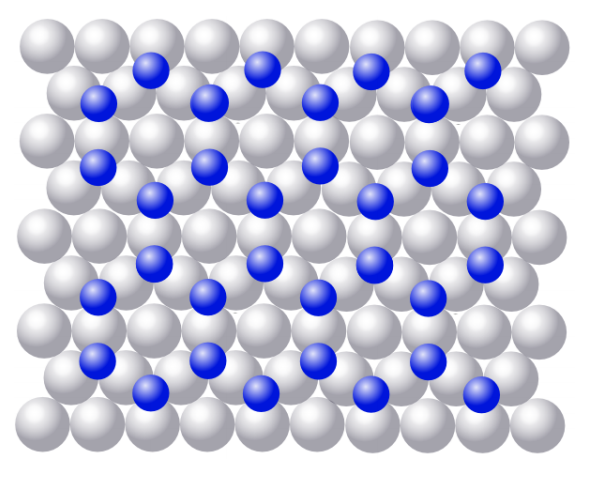
\includegraphics[width =0.9 \linewidth]{Figures/Model/Hydrogen sites.png}
        \caption{Arrangement of Hydrogen Sites
        }\label{sub@fig:hydrogen honeycomb structure}
    \end{subfigure}
    \begin{subfigure}{0.45\linewidth}
        \centering
        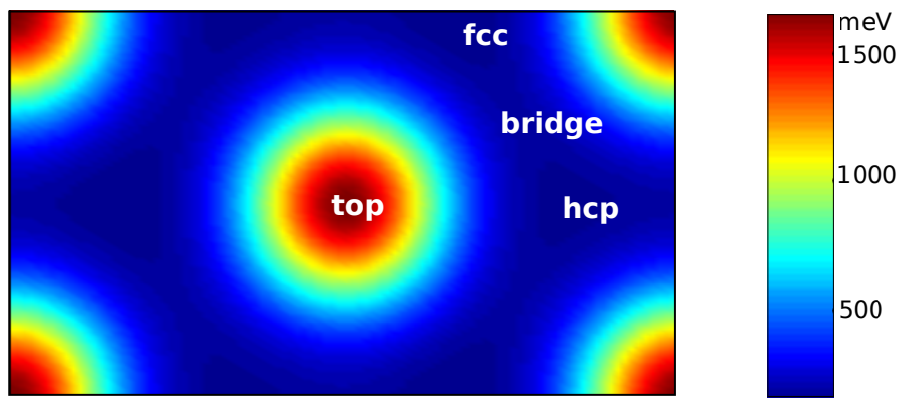
\includegraphics[width = 0.9\linewidth]{Figures/Model/Hydrogen DFT Potential.png}
        \caption{DFT Potential surface
        }\label{sub@fig:Nickel DFT surface}
    \end{subfigure}
    \caption{
        Arrangement of hydrogen
        sites on a Ni(111) surface,% ChkTeX 36
        alternating
        between low energy FCC and
        high energy HCP sites arranged
        in a honeycomb structure.
        \cref{sub@fig:hydrogen honeycomb structure,sub@fig:Nickel DFT surface}
        are reproductions of those found in\cite{Jianding-Zhu}
    }
\end{figure}
To calculate the incoherent
rate of tunneling between
the FCC and HCP ground states
we need to find a
hamiltonian to describe the combined
electron-hydrogen system.
The electron-hydrogen system can be described
by a combination of a free and interaction hamiltonian
\begin{equation}
    \hat{H} = \hat{H}_{free} + \hat{H}_{int}
\end{equation}
where the free hamiltonian \(\hat{H}_{free}\)
can be separated
into an electron and hydrogen component
\begin{equation}
    \hat{H}_{free} =
    \hat{H}_{e^-} + \hat{H}_{h}\\
\end{equation}

\subsection{Electron States}\label{sec:electron states}
Ignoring the
interaction between the electrons
and the lattice as well as electron-electron
interactions we can expand the free electron
hamiltonian in the plane wave
basis
\begin{equation}
    \hat{H}_{e^-} = \sum_{k, s}
    \frac{\hbar^2 k^2}{2m_e} \hat{b}^\dagger_{k, s} \hat{b}_{k, s}\\
\end{equation}
where \(\hat{b}^\dagger_{k, s}\)
is the electron creation operator
with spin \(s\) and wavevector
\(k\) satisfying the standard
fermion anti-commutation relations
\( \{ \hat{b}_{k, s}, \hat{b}^\dagger_{k', s'} \}
= \delta_{k k'} \delta_{s s'}\).

Taking the lattice constant of nickel as
\(3.499\pm{}0.005\times{}10^{-10}m\)~\cite{PhysRev.25.753},
we find a density of
\(9.34 \pm 0.04 \times{}10^{28}m^{-3}\).
If both of the 2 valence
electrons on nickel are completely
delocalised we
find an electron density of
\(n = 1.87\times{}10^{29} m^{-3}\).
This is used to calculate
the fermi-wavevector and fermi-energy of
nickel~\cite{KittelCharles1953Itss}
\begin{align}
    \epsilon_f & = \frac{\hbar^2}{2m} {(3\pi^2n)}^{2/3}                   \\
               & = 1.91\times{}10^{-18}J                                  \\
    k_f        & = {(3 \pi^2 n)}^{\frac{1}{3}}                            \\
               & = 1.77\times{}10^{10}m^{-1} \label{eqn:fermi wavevector}
\end{align}
From measurements of the optical
properties of nickel the
fermi energy is found to
be slightly lower
at only
\(1.24\times{} 10^{-18}J\)~\cite{PhysRev.131.2469}.

\subsection{Hydrogen States}
For hydrogen
we make use of the
eigenstates found in
the previous DFT
analysis\cite{Jianding-Zhu}.
\begin{equation}
    \hat{H}_{h} =
    E_0 \sum_{i \exists fcc} \hat{a}^\dagger_i \hat{a}_i
    + E_1 \sum_{i \exists hcp} \hat{a}^\dagger_i \hat{a}_i
\end{equation}
where \(E_0\) is the energy of an FCC site and
\(E_1\) is the energy of a HCP site.
\(\hat{a}^\dagger_i\) is
the hydrogen creation
operator for the site i
which satisfies the standard commutation
relations for a boson
\(\left[ \hat{a}_i, \hat{a}^\dagger_j \right]
= \delta_{ij}\).

Although DFT calculations
also provide a theoretical prediction
of the hydrogen energies, the
energy used in the
model were
taken from direct spin-echo measurements of the
surface\cite{Jianding-Zhu}
\begin{equation}
    \Delta{}E_{hyd} = E_1 - E_0
    = 3.04\pm0.16\times{}10^{-21} J
    \label{eqn:hydrogen energy difference}
\end{equation}


\subsection{Electron Hydrogen Interaction}
To describe the electron-hydrogen
interaction we introduce field
operators \(\hat{\psi}_e\) and
\(\hat{\psi}_h\)~\cite{nazarov_danon_2013}
\begin{equation}
    \hat{H}_{int} = \int\int{d\vec{r} d\vec{r}'
        V(\vec{r}-\vec{r}')
        \hat{\psi}^\dagger_h(\vec{r})
        \hat{\psi}^\dagger_e(\vec{r'})
        \hat{\psi}_e(\vec{r'})
        \hat{\psi}_h(\vec{r})}
\end{equation}
where \(V(\vec{r})\) is
the electron-hydrogen
interaction potential.
We expand out the
electron operator in
the free electron basis state
\begin{align}
    \hat{\psi}_e(\vec{r}) & = \sum_{k, s}
    \braket{\vec{r}|\vec{k}}
    \hat{b}_{k, s}                                      \\
                          & = \frac{1}{L^{\frac{3}{2}}}
    \sum_{k, s} \exp{(i\vec{k}.\vec{r})}
    \hat{b}_{k, s}
\end{align}
to give us the expression
\begin{align}
    \hat{H}_{int} & =
    \sum_{k, s, k', s'} \int\int{\frac{d\vec{r} d\vec{r}'}{L^3}
        V(\vec{r}-\vec{r}')
        \hat{b}^\dagger_{k',s'}
        \hat{b}_{k, s}
        \exp{(i(\vec{k} - \vec{k'}).\vec{r'})}
        \hat{\psi}^\dagger_h(\vec{r})
    \hat{\psi}_h(\vec{r})}                       \\
                  & = \begin{aligned}[t]
        \frac{1}{L^3}
        \sum_{k, s, k', s'}
         & \int d(\vec{r}' - \vec{r})
        V(\vec{r}-\vec{r}')
        \hat{b}^\dagger_{k',s'}
        \hat{b}_{k, s}
        \exp{(i(\vec{k} - \vec{k'}).(\vec{r'} - \vec{r}))} \\
         & \int d\vec{r}
        \exp{(i(\vec{k} - \vec{k'}).\vec{r})}
        \hat{\psi}^\dagger_h(\vec{r})
        \hat{\psi}_h(\vec{r})
    \end{aligned} \\
    \hat{H}_{int} & = \frac{1}{L^3}
    \sum_{k,s,k',s'}
    \hat{b}^\dagger_{k',s'}\hat{b}_{k,s}
    \tilde{V}(\vec{q})\int{d\vec{r}
    \hat{\psi}_h^{\dagger}\hat{\psi}_h
    \exp(i\vec{q}.\vec{r})}
\end{align}
If we also expand the
hydrogen creation operator
\begin{equation}
    \hat{\psi}_h(\vec{r}) =
    \sum_{i} \psi_{h,i}(\vec{r})
    \hat{a}_i
\end{equation}
we find
\begin{equation}
    \hat{H}_{int} = \frac{1}{L^3}
    \sum_{\substack{ k,s,k',s'\\ i,j}}
    \hat{b}^\dagger_{k',s'}\hat{b}_{k,s}
    \hat{a}^\dagger_i \hat{a}_k
    \tilde{V}(\vec{q})\int{d\vec{r}
        \psi^*_{h,i}(\vec{r})\psi_{h,j}(\vec{r})
        \exp(i\vec{q}.\vec{r})}\label{eqn:interaction hamiltonian expanded}
\end{equation}
where \(\vec{q} = \vec{k} - \vec{k'}\)
is the scattering wavevector, and
\(\tilde{V}(\vec{q})\) is the
fourier transform of the interaction
potential.


\subsection{The Electron Hydrogen Potential}\label{sec:electron hydrogen potential}
The interaction potential can be found from
the greens function of the coulomb
equation~\cite{AQP_Problems}
\begin{equation}
    V(\vec{r}) = \frac{e^2}{4 \pi \epsilon_0}(
    -\frac{1}{r}
    + \int{\frac{\abs{\psi(\vec{r}')}^2}{
            \abs{\vec{r} - \vec{r'}}} d\vec{r}'})
\end{equation}
Electrons surrounding the hydrogen
atom have energies
\(E_n = -\frac{13.6}{n^2} eV\)~\cite{griffiths_schroeter_2018}.
Since the energy required to excite the electron
to the \(n=2\) energy level is much greater
than the fermi energy of Ni
(\(7.76eV\))~\cite{PhysRev.131.2469} we can
make the approximation that the electron surrounding
the hydrogen lie close to the 1s ground state. This
corresponds to a wavefunction\cite{griffiths_schroeter_2018}
\begin{equation}
    \psi(\vec{r}) = {(\pi a_0^3)}^{-1/2} e^{-\frac{r}{a_0}}
\end{equation}
where \(a_0\) is
the bohr radius.
We then fourier
transform this expression
(see \cref{app:interaction potential calculation})
to find
\begin{equation}
    \tilde{V}(\vec{q}) = \frac{e^2}{\epsilon_0 q^2}(
    \frac{\alpha^4}{{(\alpha^2 + q^2)}^2} - 1
    )
\end{equation}
with \(\alpha = \frac{2}{a_0}\). If we expand
about \(q=0\) we find
\begin{align}
    \tilde{V}(q) & \sim \frac{e^2}{\epsilon_0 q^2}(1 - 2{(\frac{q}{\alpha})}^2 + 3 {(\frac{q}{\alpha})}^4 - 1)   \\
    {}           & = -\frac{2e^2}{\epsilon_0 \alpha^2}(1 - \frac{3}{2}{(\frac{q}{\alpha})}^2) + \mathcal{O}(q^4)
\end{align}
taking \(q = k_f = 1.77\times{}10^{10}m^{-1}\)
(see \cref{sec:electron states})
and \(\alpha = 3.79\times{}10^{10}\) we see the second
order correction only contributes to a variation
of around \(14.5\% \).
We therefore assume that for the relevant scattering
of electrons the potential takes a constant
value \(\tilde{V}(q) \sim -\frac{2e^2}{\epsilon_0 \alpha^2}\).

\subsection{The Hydrogen Wavefunction}
The final term in
\cref{eqn:interaction hamiltonian expanded}
involves the integral
of the product of the two
hydrogen wavefunctions.
Previous DFT calculations
gave the form of bloch wavefunctions
spread throughout the whole
material\cite{Jianding-Zhu}, so
to recover a localised wavepacket
several of these states were chosen
centered about \(q=0\).
Given the localised wavefunction
it was possible to calculate the fourier
transform products directly. The fourier transform was seen to
oscillate (\cref{fig:fourier transform oscillation})
at a frequency proportional to
\(\frac{2\pi}{a}\) where \(a\) is the lattice
constant of Ni. The value of this constant
is around
\(3.499\pm{}0.005\times{}10^{-10}m\)~\cite{PhysRev.25.753}
corresponding to oscillations at
\(q = 1.79 \pm 0.03 \times{}10^{10}m^{-1}\)
which in theory should have a noticeable
effect on the matrix element, with a
fermi wavevector of
\(1.177\times{}10^{10} m^{-1}\)~\cref{eqn:fermi wavevector}.
\begin{figure}[htbp]
    \captionsetup[subfigure]{justification=centering}
    \centering
    \begin{subfigure}{0.45\linewidth}
        \centering
        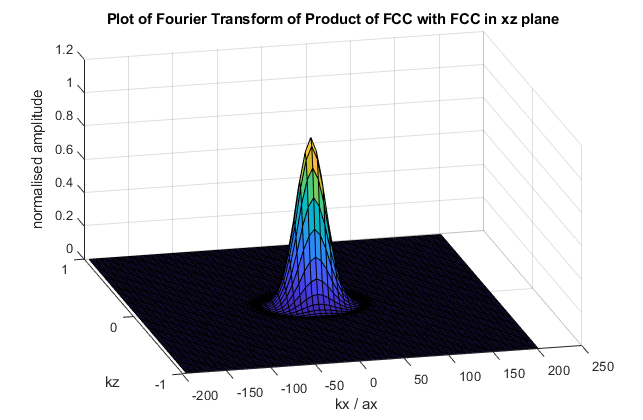
\includegraphics[width= 0.9\linewidth]{Figures/Model/Plot of fourier transform of the wavefunction fccfcc xz plane.png}
        \subcaption{FCC-FCC Fourier Transform in xz Plane}\label{fig:diagonal hydrogen matrix element no oscillation}
    \end{subfigure}
    \hfill
    \begin{subfigure}{0.45\linewidth}
        \centering
        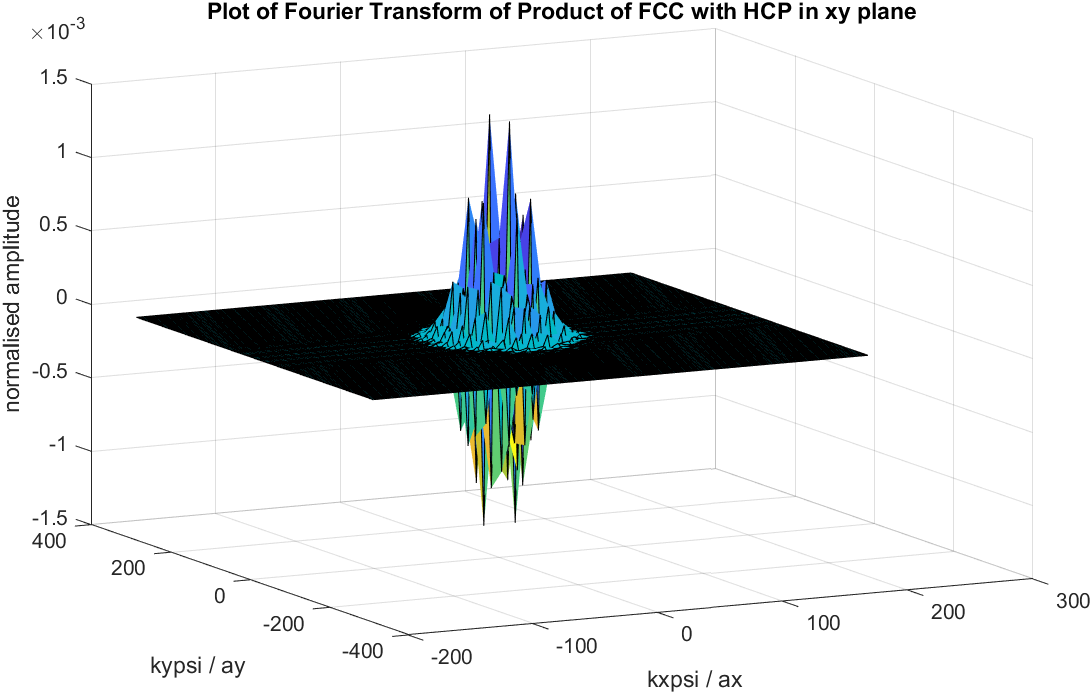
\includegraphics[width= 0.9\linewidth]{Figures/Model/Plot of fourier transform of the wavefunction.png}
        \subcaption{FCC-HCP Fourier Transform in xy Plane}\label{fig:cross hydrogen matrix element oscillation}
    \end{subfigure}
    \caption{Results of the hydrogen fourier transform calculations.
    FCC-FCC and HCP-HCP calculations
    (\cref{fig:diagonal hydrogen matrix element no oscillation})
    show a smooth curve, with a normalised
    value of \(1\) at \(q=0\).
    The FCC-HCP fourier transform
    (\cref{fig:cross hydrogen matrix element oscillation})
    however show oscillations with a characteristic
    wavevector \(q = 1.79 \pm 0.03 \times{}10^{10}m^{-1}\),
    corresponding to the lattice vector of \(Ni\).
    }\label{fig:fourier transform oscillation}
\end{figure}
In a real material
we should expect the nickel atoms
to oscillate which would break
the fixed distance between FCC and HCP
sites. The individual peaks
are therefore simply a side effect
of the DFT analysis.

Since the overall wavepacket decays over a region
of around \(\frac{100\pi}{a}\) we should be
able to ignore the oscillations of
\(V(\vec{q})\) to obtain an effective constant
potential required for the simulation. For this
model we simply take the maximum overlap
of the normalised wavefunction (\cref{tab:hydrogen overlaps}).
\begin{table}[htbp]
    \begin{center}
        \begin{tabular}{ *{3}{c} }
            \toprule
            Overlap & Maximum Overlap        & Normalised Overlap     \\
            \midrule
            FCC-FCC & \(3.00\times{}10^{7}\) & \(1\)                  \\
            HCP-HCP & \(3.00\times{}10^{7}\) & \(1\)                  \\
            HCP-FCC & \(1.33\times{}10^{5}\) & \(4.4\times{}10^{-3}\) \\
            \bottomrule
        \end{tabular}
    \end{center}
    \caption{Normalised Hydrogen overlaps as used in the
        model. Fluctuations in the overlap
        integral are ignored. The maximum
        is taken instead of the \(q=0\) value as the HCP-FCC integral
        has a minimum at this point.}\label{tab:hydrogen overlaps}
\end{table}

\subsection{Simplified Electron-Hydrogen Interaction
}\label{sec:simplified interaction}
For simplicity we introduce
an effective potential
\({\tilde{V}(\vec{q})}_{i,j}\) where
\begin{equation}
    \hat{H}_{int} = \sum_{k,s,k',s',i,j}
    {\tilde{V}(\vec{q})}_{i,j}
    \hat{b}^\dagger_{k',s'}\hat{b}_{k,s}
    \hat{a}^\dagger_{i}\hat{a}_{j}
    \label{eqn:interaction hamiltonian in k}
\end{equation}
If we take the potential to be independent
of \(q\) we can separate it
into a constant prefactor
and hydrogen overlap factors
\begin{align}
    V_{i,j}
     & =
    \frac{1}{L^3}
    \mathcal{C}_{i,j}
    \frac{2e^2}{\epsilon_0 \alpha^2} \\
     & =
    \frac{1}{L^3}
    \mathcal{C}_{i,j}
    \frac{8 \pi^2 \epsilon_0 \hbar^4}{e^2 m_e^2}
    \label{eqn:simplified interacton potential}
\end{align}
where \(\mathcal{C}\) takes
the value
\begin{align}
    \mathcal{C}_{i, i}      & = 1      \\
    \mathcal{C}_{i, \neq i} & = 0.0044
\end{align}

It is often beneficial to separate
\cref{eqn:interaction hamiltonian in k}
into a system and environment contribution.
\begin{align}
    \hat{H}_{int} & =
    \sum_{i,j}
    \hat{a}^\dagger_{i}\hat{a}_{j}
    \sum_{k,s,k',s'}
    \tilde{V}_{i,j}
    \hat{b}^\dagger_{k',s'}\hat{b}_{k,s} \\
                  & = \sum_{i,j}
    \hat{S}_{i,j} \hat{E}_{i,j}\label{eqn:split interaction hamiltonian}
\end{align}
where
\begin{align}
    \hat{S}_{i,j} & = \hat{a}^\dagger_{i}\hat{a}_{j} \\
    \hat{E}_{i,j} & = \sum_{k,s,k',s'}
    \tilde{V}_{i,j}
    \hat{b}^\dagger_{k',s'}\hat{b}_{k,s}
\end{align}